\documentclass[tikz]{standalone}
\renewcommand{\familydefault}{\sfdefault}
\begin{document}
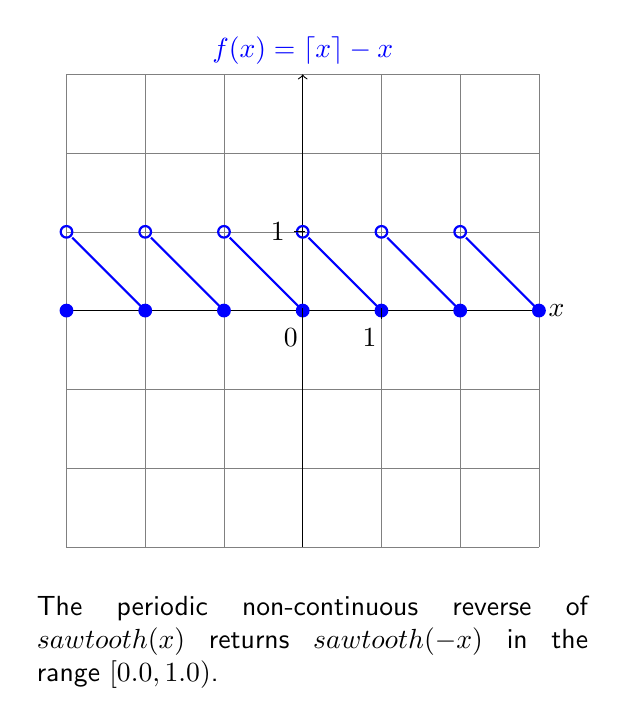
\begin{tikzpicture}
\draw [help lines] (-3,-3) grid (3,3);
\draw [->][thin] (-3, 0) -- (3, 0) node[right] {$x$};
\draw [->][thin] (0, -3) -- (0, 3) node[above, blue] {$f(x)= \left\lceil x \right\rceil - x$};

\fill [blue] (-3, 0) circle [radius=0.0735];
\draw [thick, blue] (-3, 0) circle [radius=0.0735];

\draw [thick, blue] (-2, 0) -- (-2.9265, 0.9265);
\fill [blue] (-2, 0) circle [radius=0.0735];
\draw [thick, blue] (-2, 0) circle [radius=0.0735];
\draw [thick, blue] (-3, 1) circle [radius=0.0735];

\draw [thick, blue] (-1, 0) -- (-1.9265, 0.9265);
\fill [blue] (-1, 0) circle [radius=0.0735];
\draw [thick, blue] (-1, 0) circle [radius=0.0735];
\draw [thick, blue] (-2, 1) circle [radius=0.0735];

\draw [thick, blue] (0, 0) -- (-0.9265, 0.9265);
\fill [blue] (0, 0) circle [radius=0.0735];
\draw [thick, blue] (0, 0) circle [radius=0.0735];
\draw [thick, blue] (-1, 1) circle [radius=0.0735];

\draw [thick, blue] (1, 0) -- (0.0735, 0.9265);
\fill [blue] (1, 0) circle [radius=0.0735];
\draw [thick, blue] (1, 0) circle [radius=0.0735];
\draw [thick, blue] (0, 1) circle [radius=0.0735];

\draw [thick, blue] (2, 0) -- (1.0735, 0.9265);
\fill [blue] (2, 0) circle [radius=0.0735];
\draw [thick, blue] (2, 0) circle [radius=0.0735];
\draw [thick, blue] (1, 1) circle [radius=0.0735];

\draw [thick, blue] (3, 0) -- (2.0735, 0.9265);
\fill [blue] (3, 0) circle [radius=0.0735];
\draw [thick, blue] (3, 0) circle [radius=0.0735];
\draw [thick, blue] (2, 1) circle [radius=0.0735];

\foreach \x in {0,1}
\draw (\x cm,1pt) -- (\x cm,-3pt)
    node[anchor=north,xshift=-0.15cm] {$\x$};
\foreach \y/\ytext in {1}
\draw (1pt,\y cm) -- (-3pt,\y cm) node[anchor=east] {$\ytext$};

\node[align=justify, text width=7cm, anchor=north west] at (-3.5, -3.5)
{The periodic non-continuous reverse of ${sawtooth(x)}$ returns ${sawtooth(-x)}$ in the range $[{0.0, 1.0})$.};

\end{tikzpicture}
\end{document}